\chapter{Attention Models}
First recall RNN for Captioning. It would be better if it could look the image more than once and focus its attention to specific parts of the image.

\section*{Soft Attention for Captioning}
\begin{figure}[h]
  \centering
  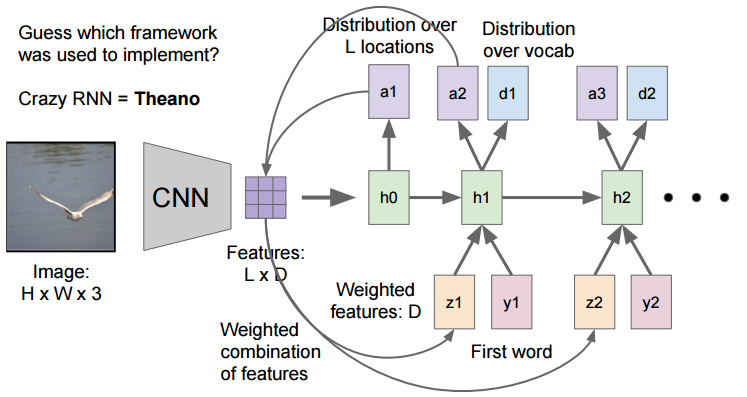
\includegraphics[width=0.7\textwidth]{Images/attention_models/1.png}
  \caption{Soft Attention for Captioning - Xu et al, “Show, Attend and Tell: Neural Image Caption Generation with Visual Attention”, ICML 2015}
\end{figure}

\begin{enumerate}
\item Compute the features with a CNN. Extract not the last ones but from an early layer. This is way it is a grid of features and not a single vector. In this way we have information of the localization of the input image features
\item Use this features to initialize the h0 hidden state
\item Now things get different with respect RNN for captioning. Instead of using h0 to compute distribution over words, we use it to compute a prob distribution over L locations. This would we implemented with a couple of affine layers (= FC) and softmax to give a distribution.
\item We produce a weighted sum of features using the prob distribution over locations. This can be seen as taking the feature vector and summarizing it to a vector. This gives as a weighted features that is used to decide where to focus.
\item The next hidden state has as inputs the past hidden state and a word (like CNN) but now we also add the weighted features.
\item The hidden state is used to produce a prob distribution over words and also a new distribution over locations. These are implemented with a couple of FC layers on top of the hidden state.
\item Go to 4
\end{enumerate}


\section*{Soft vs Hard Attention}
Lets see how this summarization vectors z are produced
\begin{figure}[h]
  \centering
  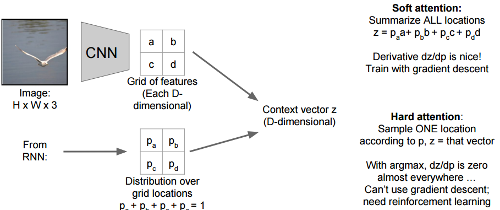
\includegraphics[width=0.7\textwidth]{Images/attention_models/2.png}
  \caption{Soft Attention vs Hard Attention}
\end{figure}

Both soft and hard attention model produce the same output. Notice that the soft attention is more diffuse because it is averaging prob from the image. And Hard attention it is only focusing in one element.

Hard attention is normally faster at test time because is only focusing on an specific thing at every step instead of looking at big regions of the image.

\begin{figure}[h]
  \centering
  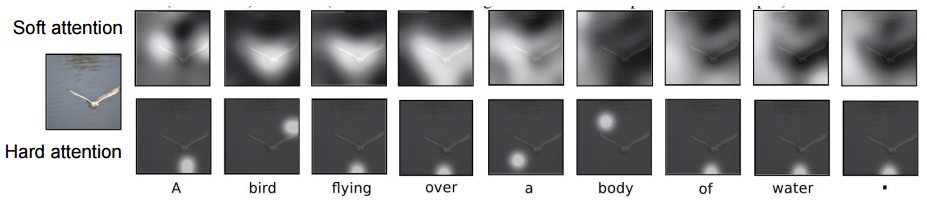
\includegraphics[width=0.7\textwidth]{Images/attention_models/3.png}
  \caption{Example Soft Attention vs Hard Attention}
\end{figure}

Both have the same problem, they are constrained by a grid  over the input image which makes them more blurry. z is not continuous. To work in a continuous way it exists the so called "Spatial Transformed Networks"


\section*{Recap}
Soft attention:
\begin{itemize}
\item Easy to implement: produce distribution over input locations, reweight features and feed as input
\item Attend to arbitrary input locations using spatial transformer networks
\end{itemize}

Hard attention:
\begin{itemize}
\item Attend to a single input location
\item Can’t use gradient descent!
\item Need reinforcement learning (because they are not differentiable)
\end{itemize}